\documentclass[a4paper, 12pt]{article}
\usepackage{geometry}
\geometry{a4paper,
total={170mm,257mm},left=2cm,right=2cm,
top=2cm,bottom=2cm}

\usepackage{mathtext}
\usepackage{amsmath}
\usepackage[T2A]{fontenc}
\usepackage[utf8]{inputenc}
\usepackage[english,russian]{babel}
\usepackage{graphicx, float}
\usepackage{tabularx, colortbl}
\usepackage{caption}
\captionsetup{labelsep=period}

\newcommand{\parag}[1]{\paragraph*{#1:}}
\DeclareSymbolFont{T2Aletters}{T2A}{cmr}{m}{it}
\newcounter{Points}
\setcounter{Points}{1}
\newcommand{\point}{\arabic{Points}. \addtocounter{Points}{1}}
\newcolumntype{C}{>{\centering\arraybackslash}X}

\author{Калинин Даниил, Б01-110}
\date{\today}
\title{Лабораторная работа 4.5.2. Интерференция лазерного излучения}

\begin{document}
\maketitle
\parindent=0cm

\parag {Цель работы}
исследовать зависимость видности интерфереционной картины от разности хода интерферирующих лучей и от их поляризации.

\parag {В работе используются}
He-Ne лазер, интерферометр Майкельсона с подвижным зеркалом, фотодиод с усилителем, осциллограф, поляроид, линейка.

\parag {Теоритическая справка} ~\\
\textbf{Лазер} \\
В лазере длиной $L$ для излучения вдоль оси для резонансных частот выполняется

\begin{equation}    
    f_m = \dfrac{c}{\lambda_m} = \dfrac{mc}{2L}.
\end{equation}

Условие генерации может выполняться для сразу нескольких колебаний с частостами $f_m$, разположенными в диапазоне генерации $2\Delta F$. В этом случае генерируется несколько волн -- \textit{мод} -- межмодовое расстояние для которых

\begin{equation}
    \label{eq:d_nu}
    \Delta \nu = f_{m+1} - f_m = \dfrac{c}{2L}.
\end{equation}

Число мод можно оценить как 
\begin{equation}
    N \approx 1 + \dfrac{2\Delta F}{\Delta \nu}.
\end{equation}

\textbf{Видность} \\ 
Видимость интерфереционной картины -- параметр, определяемый формулой

\begin{equation}
\gamma = \dfrac{I_{max} - I_{min}}{I_{max} + I_{min}},
\end{equation}

где $I_{max}$, $I_{min}$ -- максимальная и минимальная интенсивности света интерфереционной картины вблизи выбранной точки. Разобьём его на произведение функций параметров установки

$$
\gamma = \gamma_1 \gamma_2 \gamma_3.
$$

Здесь $\gamma_1$ отвечает за соотношение интенсивности интерферирующих волн:

\begin{equation}
    \label{eq:gamma1}
    \gamma_1 = \dfrac{2\sqrt{\delta}}{1+\delta},
\end{equation}

где $\delta = \frac{B_m^2}{A_m^2}$, $A_m$ и $B_m$ -- амплитуды волн. Параметр $\delta$ определяется устройством разделения волн.\\

Функция $\gamma_2$ отвечает за влияние разности хода и спектрального состава волн,

$$
\gamma_2 = \dfrac{\sum\limits_n A^2_n \cos \frac{2\pi \Delta \nu n l}{c}}{\sum\limits_n A_n^2},
$$

где $l$ -- разность хода, $\Delta \nu$ -- спектральный состав излучения, $A_n^2$ -- интенсивности мод. В непрерывном пределе получим

$$
\gamma_2 = e^{-\left(\frac{\pi \Delta F l}{c}\right)^2}
$$

-- для гауссова линии излучения с полушириной $\Delta F$ получили гауссову зависимость $\gamma_2 = \gamma_2(l)$ с полушириной 

\begin{equation}
l_{1/2} = \dfrac{c}{\pi \Delta F}\sqrt{\ln 2} \approx \dfrac{0.26 c}{\Delta F}.
\end{equation}

Последняя функция $\gamma_3$ отвечает за разность в поляризации. Если $\alpha$ -- угол между плоскостями поляризаций волн, то

\begin{equation}
    \label{eq:gamma3}
    \gamma_3 = |\cos \alpha|.
\end{equation}

\parag {Экспериментальная установка}~\\
Схема экспериментальной установки представлена на рисунке \ref{img:setup}.

\begin{figure}[h]
    \centering
    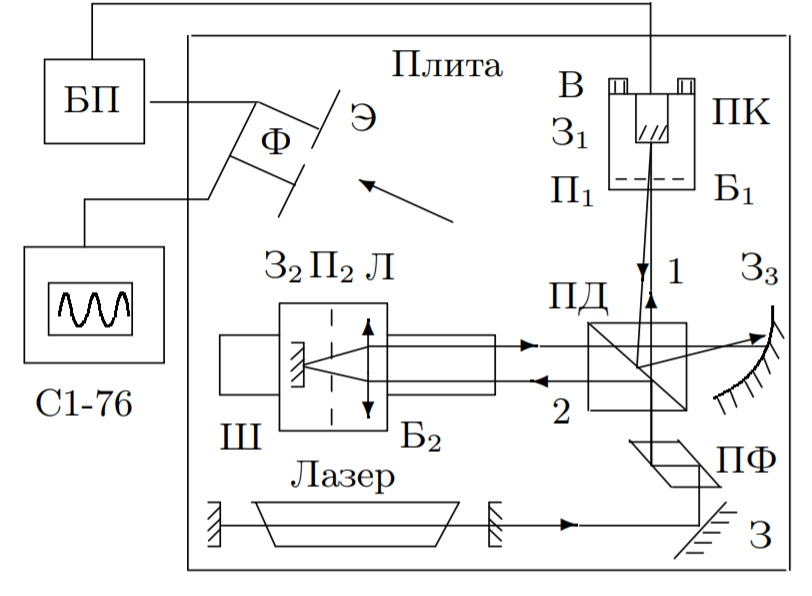
\includegraphics[scale=0.6]{setup.png}
    \caption{Схема установки}
    \label{img:setup}
\end{figure}

В работе используется интерферометр Майкельсона (рис. \ref{img:setup}). Луч лазера, отражённый от зеркала З и прошедший через параллелепипед Френеля (ПФ), делится делительной призмой ДП на два луча. Первый проходит блок $Б_1$ с поляроидом $П_1$ и зеркалом $З_1$, прикленным к пьезокерамике, которая может совершать малые колебания вдоль луча, с возможность изменения угла наклона зеркала. Второй проходит блок $Б_2$ с линзой Л, поляроидом $П_2$ и зеркалом $З_2$ в фокальной плоскости линзы, чтобы выходящий луч, в отличие от первого, был параллелен входящему. Оба луча, проходя ДП, попадают на сферическое зеркало $З_3$ и интерферируют на экране. Интенсивность света считывается фотодиодом на осциллограф через щель, параллельную интерфереционным полосам, в центре экрана. На экране осциллографа наблюдаются колебания с изменяющимся периодом, так как на пьезокерамику подаются напряжение, из-за чего её длина колеблется.

\begin{figure}
    \centering
    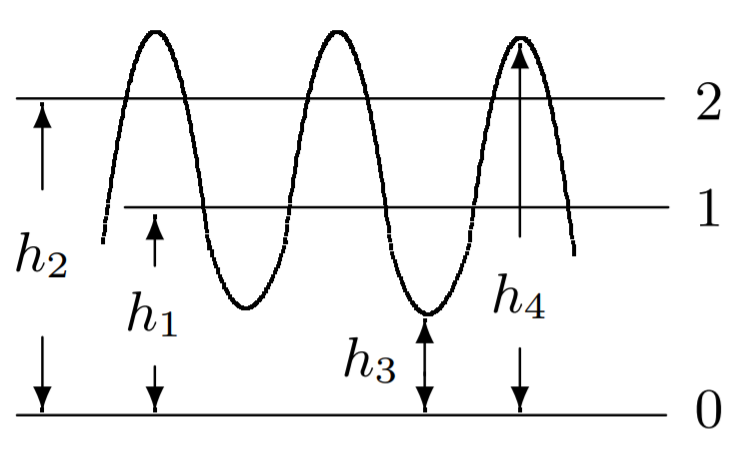
\includegraphics[scale = 0.5]{oscilograph.png}
    \caption{Осциллограмма сигналов фотодиода.}
\end{figure}

По картине на экране осциллографа можно определить параметры видимости по следующим формулам:

\begin{equation}
    \delta = \dfrac{h_1}{h_2},
\end{equation}

\begin{equation}
    \gamma = \dfrac{h_4 - h_3}{h_4 + h_3},
\end{equation}

Здесь 0 -- уровень при отсутствии лучей, 1 и 2 -- при закрытии одного из них. Используя $\delta$, можно рассчитать $\gamma_1$ по формуле \eqref{eq:gamma1}.\\ 
При условии одинаковой поляризации лучей ($\alpha = 0$),

\begin{equation}
    \gamma_2 = \dfrac{\gamma}{\gamma_1}.
\end{equation}

Если же разность хода отсутствует ($l = 0$), то
\begin{equation}
    \gamma_3 = \dfrac{\gamma}{\gamma_1}.
\end{equation}

\parag {Ход работы} ~\\

\point Изучим поляризацию лазерного луча. Введем дополнительный поляроид между лазером и РФ. Заметим, что освещение ПФ меняется в зависимости от поворота поляроида. Отсюда следует, что свет лазера поляризован линейно. Похожая картина наблюдается при размещении поляроида между РФ и ПФ, однако, при таком расположении, освещенность кубика не падает до нуля. Теперь повернем $П_1$ так, чтобы установить минимальную четкость интерференционной картины. Внесем поляроид в пучок перед экраном. При вращении поляроида вновь увидем интерференционную картину. Она возникает из-за того, что два луча вновь будут иметь одну поляризацию после прохождения внесенного поляроида. \\


\point Измерение видности. Для начала подберем положение с нулевой разностью хода. Получим, что ближайшее к нулевому значение разности хода достигается при: $h_1 = 1.1 ~ дел.$, $h_2 = 1.25 ~ дел.$, $h_3 = 0.8 ~ дел.$, $h_4 = 4.0 ~ дел.$, $\gamma_2 = 0.668$. Теперь снимем зависимость $h_1, ~ h_2, ~ h_3, ~ h_4$ от угла поляризации $\beta$. Результаты занесем в таблицу \ref{tabl:b_to_h}.


\begin{table}[h]
\centering
\begin{tabular}{|c|c|c|c|c|c|}
\hline 
    № & угол $\beta$, град. & $h_1$, дел.  & $h_2$, дел.  & $h_3$, дел.  & $h_4$, дел. \\ \hline
    1 & 114.0 & 0.35 & 1.0 & 1.35 & 1.45 \\ \hline
    2 & 103.0 & 0.15 & 1.0 & 0.9 & 1.4 \\ \hline
    3 & 95.0 & 0.1 & 1.0 & 0.8 & 1.4 \\ \hline
    4 & 87.0 & 0.1 & 0.95 & 0.75 & 1.4 \\ \hline
    5 & 80.0 & 0.5 & 0.95 & 0.7 & 1.4 \\ \hline
    6 & 70.0 & 0.1 & 0.95 & 0.6 & 1.55 \\ \hline
    7 & 60.0 & 0.1 & 0.95 & 0.6 & 1.65 \\ \hline
    8 & 50.0 & 0.15 & 0.95 & 0.5 & 1.8 \\ \hline
    9 & 40.0 & 0.25 & 0.95 & 0.45 & 2.0 \\ \hline
    10 & 30.0 & 0.45 & 0.95 & 0.5 & 2.4 \\ \hline
    11 & 25.0 & 0.55 & 1.0 & 0.55 & 2.6 \\ \hline
    12 & 15.0 & 0.6 & 1.0 & 0.6 & 2.65 \\ \hline
\end{tabular}
\caption{Зависимость видности от угла поворота поляроида при нулевой разности хода.}
\label{tabl:b_to_h}
\end{table}

Теперь, для изучения зависимости $\gamma_3(cos(\beta))$, вычислим величины $\gamma$, $\gamma_1$, $\delta$, $\gamma_3$ и $cos(\beta)$. Результаты занесем в таблицу \ref{tabl:gammas}.

\begin{table}[h]
\centering
\begin{tabular}{|c|c|c|c|c|c|c|c|c|}
\hline 
    № & угол $\beta$, град. & $cos(\beta)$ & $\sigma cos(\beta)$ & $\gamma$ & $\delta$ & $\gamma_1$ & $\gamma_3$ & $\sigma \gamma_3$ \\ \hline
    1 & 114.0 & -0.407 & 0.016 & 0.036 & 0.350 & 0.876 & 0.041  & 0.034 \\ \hline
    2 & 103.0 & -0.225 & 0.017 & 0.217 & 0.150 & 0.674 & 0.323  & 0.083 \\ \hline
    3 & 95.0 & -0.087 & 0.017 & 0.273 & 0.100 & 0.575 & 0.474  & 0.138 \\ \hline
    4 & 87.0 & 0.052 & 0.017 & 0.302 & 0.105 & 0.587 & 0.515  & 0.148 \\ \hline
    5 & 80.0 & 0.174 & 0.017 & 0.333 & 0.526 & 0.951 & 0.351  & 0.060 \\ \hline
    6 & 70.0 & 0.342 & 0.016 & 0.442 & 0.105 & 0.587 & 0.753  & 0.202 \\ \hline
    7 & 60.0 & 0.500 & 0.015 & 0.467 & 0.105 & 0.587 & 0.795  & 0.210 \\ \hline
    8 & 50.0 & 0.643 & 0.013 & 0.565 & 0.158 & 0.686 & 0.824  & 0.162 \\ \hline
    9 & 40.0 & 0.766 & 0.011 & 0.633 & 0.263 & 0.812 & 0.779  & 0.112 \\ \hline
    10 & 30.0 & 0.866 & 0.009 & 0.655 & 0.474 & 0.934 & 0.701  & 0.075 \\ \hline
    11 & 25.0 & 0.906 & 0.007 & 0.651 & 0.550 & 0.957 & 0.680  & 0.065 \\ \hline
    12 & 15.0 & 0.966 & 0.005 & 0.631 & 0.600 & 0.968 & 0.651  & 0.061 \\ \hline
    
\end{tabular}
\caption{Расчитанные коэффициенты $\gamma$, $\gamma_1$, $\delta$, $\gamma_3$ и $cos(\beta)$.}
\label{tabl:gammas}
\end{table}

Теперь построим график зависимости $\gamma_3 = \gamma_3(cos(\beta))$. Изобразим график на рисунке \ref{img:gamma_from_cos_beta}.

\begin{figure}
    \centering
    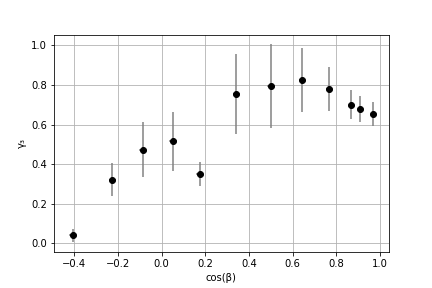
\includegraphics{gamma_from_cos_beta.png}
    \caption{График зависимости $\gamma_3(cos(\beta))$}
    \label{img:gamma_from_cos_beta}
\end{figure}

\point Теперь исследуем зависимость интерференционной картины от разности хода между лучами. Для этого будем перемещать блок $Б_2$ вдоль направления распространения луча. Координата $x$ блока будет определять разность хода. Снятые значения запишем в таблицу \ref{tabl:x_to_gammas}.

\begin{table}[h]
\centering
\begin{tabular}{|c|c|c|c|c|c|c|c|c|c|c|}
\hline 
    № &  $x$, см. & $h_1$, дел. & $h_2$, дел.  & $h_3$, дел. & $h_4$, дел. & $\gamma$ & $\delta$ & $\gamma_1$ & $\gamma_2$ & $\sigma \gamma_2$ \\ \hline
    1 & 10.5 & 1.1 & 0.85 & 0.9 & 3.1 & 0.550 & 1.294 & 0.992 & 0.555  & 0.059 \\ \hline
    2 & 10.0 & 2.2 & 2.4 & 2.4 & 4.0 & 0.250 & 0.917 & 0.999 & 0.250  & 0.021 \\ \hline
    3 & 12.0 & 2.3 & 0.8 & 2.6 & 3.8 & 0.188 & 2.875 & 0.875 & 0.214  & 0.028 \\ \hline
    4 & 14.0 & 2.2 & 1.2 & 2.3 & 4.6 & 0.333 & 1.833 & 0.956 & 0.349  & 0.028 \\ \hline
    5 & 16.0 & 2.2 & 3.2 & 4.7 & 7.0 & 0.197 & 0.688 & 0.983 & 0.200  & 0.012 \\ \hline
    6 & 18.0 & 2.2 & 1.2 & 2.6 & 4.2 & 0.235 & 1.833 & 0.956 & 0.246  & 0.023 \\ \hline
    7 & 22.0 & 2.2 & 2.2 & 3.8 & 5.2 & 0.156 & 1.000 & 1.000 & 0.156  & 0.014 \\ \hline
    8 & 26.0 & 2.2 & 3.9 & 4.8 & 5.6 & 0.077 & 0.564 & 0.960 & 0.080  & 0.011 \\ \hline
    9 & 30.0 & 2.2 & 1.0 & 3.2 & 3.3 & 0.015 & 2.200 & 0.927 & 0.017  & 0.017 \\ \hline
    10 & 36.0 & 2.2 & 2.0 & 4.2 & 4.4 & 0.023 & 1.100 & 0.999 & 0.023  & 0.012 \\ \hline
    11 & 42.0 & 2.2 & 0.6 & 2.6 & 3.2 & 0.103 & 3.667 & 0.821 & 0.126  & 0.027 \\ \hline
    12 & 46.0 & 2.2 & 1.2 & 3.4 & 3.6 & 0.029 & 1.833 & 0.956 & 0.030  & 0.015 \\ \hline
    13 & 50.0 & 2.2 & 0.8 & 3.0 & 3.0 & 0.000 & 2.750 & 0.884 & 0.000  & 0.000 \\ \hline
    14 & 56.0 & 2.4 & 0.4 & 2.6 & 2.8 & 0.037 & 6.000 & 0.700 & 0.053  & 0.029 \\ \hline
    15 & 62.0 & 2.4 & 0.4 & 2.8 & 3.0 & 0.034 & 6.000 & 0.700 & 0.049  & 0.027 \\ \hline
    16 & 64.0 & 2.4 & 0.4 & 2.6 & 3.0 & 0.071 & 6.000 & 0.700 & 0.102  & 0.032 \\ \hline
    17 & 66.0 & 2.4 & 0.4 & 2.6 & 3.2 & 0.103 & 6.000 & 0.700 & 0.148  & 0.037 \\ \hline
    18 & 70.0 & 2.4 & 0.4 & 2.8 & 3.2 & 0.067 & 6.000 & 0.700 & 0.095  & 0.030 \\ \hline
    19 & 74.0 & 2.4 & 0.8 & 2.6 & 4.0 & 0.212 & 3.000 & 0.866 & 0.245  & 0.029 \\ \hline
    20 & 76.0 & 2.5 & 1.0 & 2.7 & 4.3 & 0.229 & 2.500 & 0.904 & 0.253  & 0.026 \\ \hline
    21 & 78.0 & 2.8 & 1.2 & 3.2 & 4.6 & 0.179 & 2.333 & 0.917 & 0.196  & 0.020 \\ \hline
    22 & 82.0 & 3.2 & 1.6 & 4.4 & 5.2 & 0.083 & 2.000 & 0.943 & 0.088  & 0.012 \\ \hline
    23 & 88.0 & 3.4 & 2.2 & 3.4 & 4.0 & 0.081 & 1.545 & 0.977 & 0.083  & 0.015 \\ \hline
    
\end{tabular}
\caption{Зависимость $\gamma_2$ от разности хода.}
\label{tabl:x_to_gammas}
\end{table}


По полученным данным построим график зависимости $\gamma_2(x)$, изображенный на рисунке \ref{img:gamma_from_x}

\begin{figure}
    \centering
    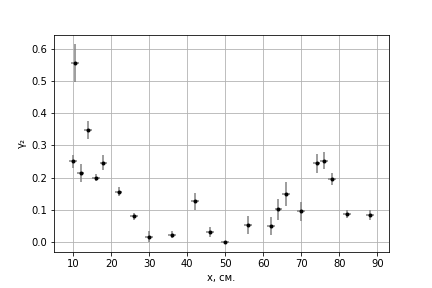
\includegraphics{gamma_from_x.png}
    \caption{График зависимости $\gamma_2(x)$}
    \label{img:gamma_from_x}
\end{figure}

На полученном графике видно два максимума: при $x_1 = 14 \pm 2$ см. и $x_2 = 76 \pm 2$ см.  Тогда $L = \frac{1}{2}(x_2 - x_1) = 31.0 \pm 1.4 \text{ см}$. Отсюда из формулы \eqref{eq:d_nu}

$$
\Delta \nu = \dfrac{c}{2L} = (4.84 \pm 0.2) \cdot 10^8 \text{ Гц}.
$$

\point Определим полуширину главного максимума по уровню $\approx \gamma_2$. Рассмотрим вертикали до границы "купола" через пиковую точку и получим: $l_{\frac{1}{2}} = 7.8 \pm 0.9$ см.

\point Определим диапазон частот, в которых происходит генерация продольных мод:
$\Delta \nu_{полн.} = (2.31 \pm 0.27) \cdot 10^9$ Гц.

\point Оценим число продольных мод, генерируемых лазером:
$ n = (5.8 \pm 0.8) \Rightarrow n \in \{5; 6\}$

\parag {Заключение} ~\\
В работе была изучена видность интерференционной картины от угла поворота поляроида: $\gamma_3(cos(\beta))$, также была изучена зависимость интерференционной картины от разности хода между лучами: $\gamma_2(x)$, определено расстояние $L$ между зеркалами оптического резонатора, а также получено межмодовое расстояние $\Delta \nu$.

\end{document}
